\documentclass[12pt,letterpaper,oneside]{book} 
%\documentclass[12pt,twoside,letterpaper]{book}
% oneside indica que nao � frente e verso

% ---------------------------------------------------------------------------- %
% Pacotes 
\usepackage[T1]{fontenc}
\usepackage[brazil]{babel}
\usepackage[latin1]{inputenc}
\usepackage[pdftex]{graphicx}           % usamos arquivos pdf/png como figuras
\usepackage{setspace}                   % espa�amento flex�vel
\usepackage{indentfirst}                % indenta��o do primeiro par�grafo
\usepackage{makeidx}                    % �ndice remissivo
\usepackage[nottoc]{tocbibind}          % acrescentamos a bibliografia/indice/conteudo no Table of Contents
\usepackage{courier}                    % usa o Adobe Courier no lugar de Computer Modern Typewriter
\usepackage{type1cm}                    % fontes realmente escal�veis
\usepackage{listings}                   % para formatar c�digo-fonte (ex. em Java)
\usepackage{titletoc}
%\usepackage[bf,small,compact]{titlesec} % cabe�alhos dos t�tulos: menores e compactos
\usepackage[fixlanguage]{babelbib}
\usepackage[font=small,format=plain,labelfont=bf,up,textfont=it,up]{caption}
\usepackage[usenames,svgnames,dvipsnames]{xcolor}
\usepackage[a4paper,top=2.54cm,bottom=2.0cm,left=2.0cm,right=2.54cm]{geometry} % margens
%\usepackage[pdftex,plainpages=false,pdfpagelabels,pagebackref,colorlinks=true,citecolor=black,linkcolor=black,urlcolor=black,filecolor=black,bookmarksopen=true]{hyperref} % links em preto
\usepackage[pdftex,plainpages=false,pdfpagelabels,pagebackref,colorlinks=true,citecolor=DarkGreen,linkcolor=NavyBlue,urlcolor=DarkRed,filecolor=green,bookmarksopen=true]{hyperref} % links coloridos
\usepackage[all]{hypcap}                    % soluciona o problema com o hyperref e capitulos
\usepackage[round,sort,nonamebreak]{natbib} % cita��o bibliogr�fica textual(plainnat-ime.bst)
\fontsize{60}{62}\usefont{OT1}{cmr}{m}{n}{\selectfont}

% By David
\usepackage[dvips]{graphicx} 
\usepackage{amsthm}
\usepackage{acronym} 
\usepackage[portugues,ruled,vlined,linesnumbered]{algorithm2e/algorithm2e}
\usepackage{supertabular}

\makeindex  % <== Talvez seja desnecessario

\pagestyle{headings}
\markboth{}{}

% ---------------------------------------------------------------------------- %
% Dimens�es da p�gina (letterpaper)
%\setlength{\paperwidth}{216mm}
%\setlength{\topmargin}{1.3cm}         % deslocamento do topo do texto 
%\setlength\oddsidemargin{0cm}
%\setlength\evensidemargin{0cm}
%\setlength{\parskip}{1.2mm}
%\setlength{\parindent}{4mm}
%\setlength{\textwidth}{135mm}          % largura do texto
%\setlength{\parindent}{0pt}
%\setlength{\textheight}{22cm}
%\setlength{\parskip}{0.2cm}


\newcommand{\eb}{\varepsilon}
\newcommand{\mdp}{\langle\mathcal{S,A},p,r,c\rangle}
\newcommand{\ctlstar}{{\sc ctl}$^\star$}
\newcommand{\ctl}{\sc ctl}
\newcommand{\ltl}{\sc ltl}
\newtheorem{Def}{Defini��o}[chapter]
\newtheorem{Teo}{Teorema}[chapter]
\newtheorem{Ex}{Exemplo}[section]
\newtheorem{Tab}{Tabela}[chapter]

\begin{document}
%\hypersetup{
%pdfauthor = {Suelen Goularte Carvalho},
%pdftitle = {Algo Relacionado a Mobile},
%pdfsubject = {Disserta��o de Mestrado},
%pdfkeywords={Mobile, Computa��o Movel, Celular} % <== Precisa rever o que vai colocar aqui !!!
%pdfcreator = {LaTeX with hyperref package},
%}

\frontmatter

\onehalfspacing
\thispagestyle{empty}
\begin{center}
    \vspace*{0.2cm}
    \textbf{\Large{Um conjunto validado de code-smells em Arquiteturas Model-View-Controller no ambiente Android a ser apresentado � CPG para a disserta��o}}\\
	
    \vspace*{1.2cm}
    \Large{Suelen Goularte Carvalho} \\ 
    
    \vskip 2cm
	\textsc{
	Disserta��o apresentada\\[-0.25cm] 
	ao\\[-0.25cm]
	Instituto de Matem�tica e Estat�stica\\[-0.25cm]
	da\\[-0.25cm]
	Universidade de S�o Paulo\\[-0.25cm]
	para\\[-0.25cm]
	obten��o do t�tulo\\[-0.25cm]
	de\\[-0.25cm]
	Mestre em Ci�ncias}
    
    \vskip 1.5cm
    Programa: Ci�ncia da Computa��o\\
    Orientador: Prof. Dr. Marco Aur�lio Gerosa\\

    \vskip 1.5cm
    �rea de Concentra��o: Computa��o M�vel\\
    Orientador: Prof. Dr. Marco Aur�lio Gerosa\\

    \vskip 1cm
	\normalsize{}
	
    \vskip 0.5cm
    \normalsize{S�o Paulo, Julho de 2016}

\end{center}

% P�gina de rosto
\newpage
\thispagestyle{empty}
	\begin{center}
    	\vspace*{0.2 cm}
        \textbf{\Large{Um conjunto validado de code-smells em Arquiteturas Model-View-Controller no ambiente Android a ser apresentado � CPG para disserta��o}}\\
	    \vspace*{2 cm}
	\end{center}

	\vskip 2cm

	\begin{flushright}
	Esta � a vers�o original da disserta��o elaborada pelo\\
	candidato Suelen Goularte Carvalho, tal como\\
	submetida a Comiss�o Julgadora.\\
	\vskip 3cm

	\end{flushright}
	\vskip 4.2cm

	\begin{quote}
	\noindent Comiss�o Julgadora:
	
	\begin{itemize}
		\item {Prof. Dr. Marco Aur�lio Gerosa $-$ IME-USP}
		\item {Prof. Dr. Nome 222 222 $-$ IME-USP}
		\item {Prof. Dr. Nome 333 333 $-$ IME-USP}
	\end{itemize}
	  
	\end{quote}

\newpage
\thispagestyle{empty}
	\vspace*{12cm}
	\vskip 1cm

	\begin{flushright}
	{\small Dedico esta disserta��o de mestrado aos meus\\
	\ldots \\
	\ldots \\
	\ldots .\\}
	\end{flushright}

	\vspace*{1cm}

	\begin{flushright}
	%{\it ``A Estrada vai sempre em frente''} \\
	%$-$ Bilbo Baggins
	\end{flushright}

\pagebreak


\pagenumbering{roman}

\onehalfspacing
\chapter*{Agradecimentos}
\setlength{\parindent}{0mm}

Lorem ipsum dolor sit amet, consectetur adipiscing elit, sed do eiusmod tempor incididunt ut labore et dolore magna aliqua. Ut enim ad minim veniam, quis nostrud exercitation ullamco laboris nisi ut aliquip ex ea commodo consequat. Duis aute irure dolor in reprehenderit in voluptate velit esse cillum dolore eu fugiat nulla pariatur. Excepteur sint occaecat cupidatat non proident, sunt in culpa qui officia deserunt mollit anim id est laborum. \\

Lorem ipsum dolor sit amet, consectetur adipiscing elit, sed do eiusmod tempor incididunt ut labore et dolore magna aliqua. Ut enim ad minim veniam, quis nostrud exercitation ullamco laboris nisi ut aliquip ex ea commodo consequat. \\
%; e a todos os outros que de alguma forma contribu�ram para este momento. \\

%Agrade�o primeiramente
Lorem ipsum dolor sit amet, consectetur adipiscing elit, sed do eiusmod tempor incididunt ut labore et dolore magna aliqua.  \\

Lorem ipsum dolor sit amet, consectetur adipiscing elit, sed do eiusmod tempor incididunt ut labore et dolore magna aliqua. \\

Lorem ipsum dolor sit amet, consectetur adipiscing elit, sed do eiusmod tempor incididunt ut labore et dolore magna aliqua. \\

%%%%%%%%%%%%%%%%%%%%%%%%%%%%%%%%%%%%%%%%%%%%%%%%%%%%%%%%%%%%%%%%%%%%%%%
\setlength{\parindent}{0pt}
\setlength{\textheight}{22cm}
\setlength{\parskip}{0.2cm}

% Para aumentar o espa�amento entre as linhas
\linespread{1.2}
%%%%%%%%%%%%%%%%%%%%%%%%%%%%%%%%%%%%%%%%%%%%%%%%%%%%%%%%%%%%%%%%%%%%%%%

\chapter*{Resumo}

Lorem ipsum dolor sit amet, consectetur adipiscing elit, sed do eiusmod tempor incididunt ut labore et dolore magna aliqua. Ut enim ad minim veniam, quis nostrud exercitation ullamco laboris nisi ut aliquip ex ea commodo consequat. Duis aute irure dolor in reprehenderit in voluptate velit esse cillum dolore eu fugiat nulla pariatur. Excepteur sint occaecat cupidatat non proident, sunt in culpa qui officia deserunt mollit anim id est laborum. \\

Lorem ipsum dolor sit amet, consectetur adipiscing elit, sed do eiusmod tempor incididunt ut labore et dolore magna aliqua. Ut enim ad minim veniam, quis nostrud exercitation ullamco laboris nisi ut aliquip ex ea commodo consequat. \\

Lorem ipsum dolor sit amet, consectetur adipiscing elit, sed do eiusmod tempor incididunt ut labore et dolore magna aliqua. Ut enim ad minim veniam, quis nostrud exercitation ullamco laboris nisi ut aliquip ex ea commodo consequat. Duis aute irure dolor in reprehenderit in voluptate velit esse cillum dolore eu fugiat nulla pariatur. Excepteur sint occaecat cupidatat non proident, sunt in culpa qui officia deserunt mollit anim id est laborum. \\

Lorem ipsum dolor sit amet, consectetur adipiscing elit, sed do eiusmod tempor incididunt ut labore et dolore magna aliqua. Ut enim ad minim veniam, quis nostrud exercitation ullamco laboris nisi ut aliquip ex ea commodo consequat. Duis aute irure dolor in reprehenderit in voluptate velit esse cillum dolore eu fugiat nulla pariatur. Excepteur sint occaecat cupidatat non proident, sunt in culpa qui officia deserunt mollit anim id est laborum. \\

%\cleardoublepage
\noindent \textbf{Palavras-chave:} planejamento em Intelig�ncia Artificial, reparo de plano, replanejamento.

\chapter*{Abstract}

Lorem ipsum dolor sit amet, consectetur adipiscing elit, sed do eiusmod tempor incididunt ut labore et dolore magna aliqua. Ut enim ad minim veniam, quis nostrud exercitation ullamco laboris nisi ut aliquip ex ea commodo consequat. Duis aute irure dolor in reprehenderit in voluptate velit esse cillum dolore eu fugiat nulla pariatur. Excepteur sint occaecat cupidatat non proident, sunt in culpa qui officia deserunt mollit anim id est laborum. \\

Lorem ipsum dolor sit amet, consectetur adipiscing elit, sed do eiusmod tempor incididunt ut labore et dolore magna aliqua. Ut enim ad minim veniam, quis nostrud exercitation ullamco laboris nisi ut aliquip ex ea commodo consequat. \\

Lorem ipsum dolor sit amet, consectetur adipiscing elit, sed do eiusmod tempor incididunt ut labore et dolore magna aliqua. Ut enim ad minim veniam, quis nostrud exercitation ullamco laboris nisi ut aliquip ex ea commodo consequat. Duis aute irure dolor in reprehenderit in voluptate velit esse cillum dolore eu fugiat nulla pariatur. Excepteur sint occaecat cupidatat non proident, sunt in culpa qui officia deserunt mollit anim id est laborum. \\

Lorem ipsum dolor sit amet, consectetur adipiscing elit, sed do eiusmod tempor incididunt ut labore et dolore magna aliqua. Ut enim ad minim veniam, quis nostrud exercitation ullamco laboris nisi ut aliquip ex ea commodo consequat. Duis aute irure dolor in reprehenderit in voluptate velit esse cillum dolore eu fugiat nulla pariatur. Excepteur sint occaecat cupidatat non proident, sunt in culpa qui officia deserunt mollit anim id est laborum. \\

\noindent \textbf{Keywords:} Artificial Intelligence planning, plan repair, replanning.

\onehalfspacing
\tableofcontents

\chapter{Lista de Abreviaturas}

\begin{acronym}

\acro{ADL}{{\it Action Description Language}} % 
\acro{AIPS}{{\it International Artificial Intelligence Planning Systems}}
\acro{BDD}{{\it Binary Decision Diagram}} %  
\acro{CGP}{{\it Conformant Graphplan}} %
\acro{CSP}{{\it Constraint Satisfaction Problems}}
\acro{CWA}{{\it Closed World Assumption}}
\acro{GPG}{{\it Greedy Planning Graph}} %  
\acro{GPS}{{\it General Problem Solver}}
\acro{HTN}{{\it Hierarchical Task Network}} %  
\acro{IPEM}{{\it Integrated Planning, Exe\-cu\-ti\-on, and Mo\-ni\-to\-ring}} %  
\acro{MDP}{{\it Markov Decision Process}} % 
\acro{PDDL}{{\it Problem Domain Definition Language}} %  
\acro{POCL}{{\it Partial Order Causal Link}}
\acro{POMDP}{{\it Partially Observable Markov Decision Process}} % 
\acro{POP}{{\it Partial Order Planner}} %  
\acro{POPR}{{\it Partial Order Plan Repair}} %  
\acro{PRM}{{\it Probabilistic Roadmap Method}} % 
\acro{SIPE}{{\it System for Iteractive Planning and Exe\-cu\-ti\-on Mo\-ni\-to\-ring}} % 
\acro{STN}{{\it Simple Temporal Netwaorking}}
\acro{STRIPS}{{\it Stanford Research Institute Planning System}} % 
\acro{UCPOP}{{\it Partial Order Planner whose step descriptions include Conditional effects and Universal quantification}}
\acro{VHPOP}{{\it Versatile Heuristic Partial Order Planner}}
%\acro{VHPOP-RE}{VHPOP-RE}


%\acro{ADL}{Linguagem de Descri��o de A��o ({\it Action Description Language})} % 
%\acro{AIPS}{Sistemas de Planejamento em Intelig�ncia Artificial ({\it Artificial Intelligence Planning Systems}) }
%\acro{BDD}{Diagrama de Decis�o Bin�ria ({\it Binary Decision Diagram})} %  
%\acro{CGP}{Grafo de Planejamento Conformante ({\it Conformant Graphplan})} %
%\acro{CPU}{Unidade Central de Processamento ({\it Central Processing Unit})}
%\acro{CSP}{Problemas de Satisfa��o de Restri��es ({\it Constraint Satisfaction Problems})}
%\acro{CWA}{Suposi��o de Mundo Fechado ({\it Closed World Assumption})}
%\acro{GPG}{Grafo de Planejamento Guloso ({\it Greedy Planning Graph})} %  
%\acro{GPS}{Solucionador de Problemas Gen�rico ({\it General Problem Solver})}
%\acro{HTML}{Linguagem de Marca��o de Hipertexto ({\it HyperText Markup Language})}
%\acro{HTN}{Rede Hier�rquica de Tarefas ({\it Hierarchical Task Network})} %  
%\acro{IA}{Intelig�ncia Artificial ({\it Artificial Intelligence})} % 
%% ATEN��O: Na dissertacao nao foi utilizado ``\ac{IA}'' pois nao se desejava que a versao em EN estivesse no texto
%\acro{IPEM}{Planejamento Integrado, Execu��o, e Monitoramento ({\it Integrated Planning, Exe\-cu\-ti\-on, and %Mo\-ni\-to\-ring})} %  
%\acro{MDP}{Processo de Decis�o de Markov ({\it Markov Decision Process})} % 
%\acro{PDDL}{Linguagem de Defini��o de Dom�nio de Planejamento ({\it Problem Domain Definition Language})} %  
%% ATEN��O: Na maior parte disserta��o nao foi utilizado ``\ac{PDDL}'' pois nao se desejava que a versao em PT-BR estivesse no %texto. 
% Somente no Ap�ndice deve aparece a verao por extenso
%\acro{POCL}{V�nculos Causais em Ordem Parcial ({\it Partial Order Causal Link})}
%% ATEN��O: Na disserta��o nao foi utilizado ``\ac{POCL}'' pois se desejava mostrar a sigla em outro formato
%\acro{POMDP}{Processo de Decis�o de Markov Parcialmente Observ�vel ({\it Partially Observable Markov Decision Process})} % 
%\acro{POP}{Planejador de Ordem Parcial ({\it Partial Order Planner})} %  
%\acro{POPR}{Reparo de Plano de Ordem Parcial ({\it Partial Order Plan Repair})} %  
%\acro{PRM}{M�todo Probabil�stico de Roteiro ({\it Probabilistic Roadmap Method})} % 
%\acro{RAM}{Mem�ria de Acesso Aleat�rio ({\it Random Access Memory})}
%\acro{SIPE}{Sistema para Planejamento Iterativo e Monitoramento de Execu��o ({\it System for Iteractive Planning and %Exe\-cu\-ti\-on Mo\-ni\-to\-ring})} % 
%\acro{STN}{Rede Temporal Simples ({\it Simple Temporal Netwaorking})}
%\acro{STRIPS}{Instituto Stanford de Pesquisa em Sistemas de Planejamento ({\it Stanford Research Institute Planning System})} %% 
%% ATEN��O: Na dissertacao nao foi utilizado ``\ac{STRIPS}'' pois nao se desejava que a versao em PT-BR estivesse no texto
%\acro{UCPOP}{Planejador de Ordem Parcial com efeitos Condicionais e quantifica��o Universal ({\it Partial Order Planner whose %step descriptions include Conditional effects and Universal quantification})}
%% ATEN��O: Na disserta��o nao foi utilizado ``\ac{UCPOP}'' pois nao se desejava que a versao em PT-BR estivesse no texto
%\acro{UML}{Linguagem de Modelagem Unificada ({\it Unified Modeling Language})}
%\acro{VHPOP}{Planejador de Ordem Parcial com Versatilidade Heur�stica ({\it Versatile Heuristic Partial Order Planner})}
%%\acro{VHPOP-RE}{VHPOP-RE}

\end{acronym}


\chapter{Lista de S�mbolos}

\begin{supertabular}{ll}


$\Sigma$ & Sistema de transi��o de estados \\
$\Sigma'$ & Sistema de transi��o de estados restrito (est�tico e determin�stico) \\
$\Pi$ & Problema de planejamento \\

$\epsilon$ & Evento nulo \\
$\eta$ & Fun��o de observa��o \\
$\gamma$ & Fun��o de transi��o de estados \\
$\gamma(s, a)$ & Progress�o, conjunto de estados resultantes da aplica��o de $a$ a $s$ \\
$\gamma^{-1}(s, a)$ & Regress�o, conjunto de estados que levam a $s$ com a aplica��o de $a$ \\
$\pi$ & Plano \\

$2^S$ & Conjunto pot�ncia de $S$ \\

$\mathcal{A}$ & Conjunto de todas as a��es poss�veis \\
$\mathcal{C}$ & Conjunto de s�mbolos de constantes \\
$\mathcal{D}$ & Dom�nio de planejamento, conjunto de operadores \\
$\mathcal{E}$ & Conjunto de eventos \\
$\mathcal{H}$ & Hist�rico de refinamentos \\
$\mathcal{O}$ & Conjunto de todas as observa��es poss�veis \\
$\mathcal{P}$ & Plano parcial \\
$\mathcal{R}$ & Estrat�gia de refinamento \\
$\mathcal{S}$ & Conjunto de todos os estados poss�veis \\

$E_p$ & Estrutura do plano \\
$G$ & Conjunto de estados meta \\
$O$ & Conjunto de observa��es, sub-conjunto de $\mathcal{S}$ \\
$P$ & Problema de planejamento \\
$S$ & Conjunto de estados, sub-conjunto de $\mathcal{S}$ \\
$S_0$ & Conjunto de estados iniciais \\
$S_g$ & Conjunto de estados objetivos \\

$\mathsf{no\mbox{-}op}$ & A��o nula \\

$a$ & A��o de $\mathcal{A}$ \\
$e$ & Evento de $\mathcal{E}$\\

$o$ & Observa��o de $\mathcal{O}$ \\
$s$ & Estado de $\mathcal{S}$ \\
$s_0$ & Estado inicial \\

%$\langle \ldots \rangle$ & tupla \\
%$( \ldots )$ & lista \\
%$\{ \ldots \}$ & conjunto \\
%
%$\cup$ & uni�o de conjuntos \\
%$\cap$ & interse��o de conjuntos \\
%$\setminus$ & subtra��o de conjuntos \\


\end{supertabular}


\listoffigures
\listofalgorithms

\mainmatter

%%%%%%%%%%%%%%%%%%%%%%%%%%%%%%%%%%%%%%%%%%%%%%%%%%%%%%%%%%%%%%%%%%%%%%%%%
\onehalfspacing

% -*- root: dissertacao.tex -*-
%%%%%%%%%%%%%%%%%%%%%%%%%%%%%%%%%%%%%%%%%%%%%%%%%%%%%%%%%%%%%%%%%%%%%%%
\setlength{\parindent}{0pt}
\setlength{\textheight}{22cm}
\setlength{\parskip}{0.2cm}

% Para aumentar o espa�amento entre as linhas
\linespread{1.2}
%%%%%%%%%%%%%%%%%%%%%%%%%%%%%%%%%%%%%%%%%%%%%%%%%%%%%%%%%%%%%%%%%%%%%%%

\chapter{Introdu��o}


\textit{``Qualquer tolo consegue escrever c�digo que um computador consegue entender. Bons programadores conseguem escrever c�digo que humanos conseguem entender''} \cite{1999:RID:311424} � uma cita��o popular conhecida por desenvolvedores. De fato, escrever c�digo de f�cil manuten��o pode ser desafiador. Por este motivo � comum desenvolvedores seguirem boas pr�ticas de programa��o j� estabelecidas \cite{FinavaroAniche2016}. Apesar de estas boas pr�ticas ajudarem a mitigar o decl�nio da quaidade de c�digo, na pr�tica � dif�cil escrever \textit{``c�digo limpo''}. 


Tal como qualquer projeto de software, ao se implementar um aplicativo Android, buscamos escrever um c�digo de qualidade e de f�cil manuten��o. De fato esta � uma tarefa desafiadora em qualquer projeto e por isso diversos estudos e livros j� foram publicados sobre esta tem�tica. � comum se aplicar boas pr�ticas de software consolidadas para projetos Java em projetos Android, devido a ambos se utilizarem da mesma linguagem e parad�gmas. No entanto, projetos Android trazem um desafio a mais, e diferentemente de outros projetos de software eles possuem algumas particularidades com rela��o a camada de apresenta��o. A estrutura de projetos Android se resume a um dir�torio \textit{java} onde ficam as classes java, um arquivo de configura��o chamado \textit{AndroidManifest.xml} que cont�m configura��es tais como primeira tela, permiss�es dentre outros e um diret�rio chamado \textit{res}, abrevia��o para o termo \textit{resources}, que cont�m subpastas com nomes pr�-determinados pelo Android, onde cada subpasta cont�m arquivos que desempenham pap�is espec�ficos na aplica��o. Por exemplo a subpasta \textit{layout} cont�m arquivos que representam a parte visual de telas do Android, a subpasta \textit{drawable} cont�m os elementos gr�ficos, por exemplo, imagens. J� a sub-pasta 


\section{Motiva��o}\index{motiva��o}

Smartphones existem desde 1993 por�m nesta �poca o foco era voltado para empresas e suas necessidades. Em 2007 houve o lan�amento do iPhone fabricado pela Apple, o primeiro smartphone voltado ao p�blico em geral. Ao final do mesmo ano o Google revelou seu sistema operacional para dispositivos m�veis, o Android \cite{SmartSociety:13}.

Nos anos que se seguiram diversas grandes empresas como Apple, Google, Blackberry e Microsoft entraram no mercado de smartphones e sistemas operacionais m�veis. Desde ent�o a ado��o do uso de smartphones e mais recentemente outros dispositivos m�veis conhecidos como dispositivos m�veis vest�veis (do ingl�s \textit{wearables}) tais como rel�gios inteligentes, pulseiras, dentre outros, tem crescido espantosamente.

Dentro do mercado de smartphone o Android tem ganhado for�a, o que resulta em mais pessoas usando dispositivos rodando aplica��es android. Desta forma, a demanda por aplicativos tem aumentado de forma acentuada. Logo, a quantidade de aplicativos desenvolvidos tem aumentado em propor��es similares. Isso significa que mais e mais projetos de aplicativos Android vem sendo constru�dos. 

Este crescimento de projetos de aplicativos na plataforma m�vel Android despertou a necessidade e interesse em explorar em mais profundidade quais s�o as particularidades de desenvolvimento nesta plataforma. Este trabalho vem contribuir com uma cole��o de \textit{code smells} validados, particulares a plataforma Android. 
 \\


\section{Objetivos}

A fazer. \\


\section{Abordagem de Solu��o}\index{abordagem}

A fazer. \\


\section{Originalidade e Relev�ncia}\index{originalidade}

H� muitos anos pesquisas em torno de maus cheiros de c�digo s�o realizadas. J� existem inclusive diversos maus cheiros mapeados, por�m poucos deles s�o feitos com rela��o a aplicativos Android nativos. Segundo artigos recentes [][] o estudo sobre maus cheiros de c�digo sobre aplicativos Android ainda est�o em sua inf�ncia, por�m ainda assim s�o muito relevantes inclusive notando-se que � mais comum identificar em aplicativos Android maus cheiros mapeados exclusivamente para esta plataforma do que os maus cheiros tradicionais. \\

Apesar de alguns esfor�os j� realizados neste sentido, a maior parte dos maus cheiros identificados espec�ficamente sobre a plataforma Android s�o espec�ficos sobre desempenho, economia de energia ou alguma outra caracter�stica que beneficie de alguma forma a experi�ncia do usu�rio, e n�o a qualidade e manuten��o de c�digo.


\section{Organiza��o do Trabalho}\index{organiza��o}

A fazer. \\

 
%%%%%%%%%%%%%%%%%%%%%%%%%%%%%%%%%%%%%%%%%%%%%%%%%%%%%%%%%%%%%%%%%%%%%%%
\setlength{\parindent}{0pt}
\setlength{\textheight}{22cm}
\setlength{\parskip}{0.2cm}

% Para aumentar o espa�amento entre as linhas
\linespread{1.2}
%%%%%%%%%%%%%%%%%%%%%%%%%%%%%%%%%%%%%%%%%%%%%%%%%%%%%%%%%%%%%%%%%%%%%%%

\chapter{Fundamenta��o Te�rica}

Planejamento\index{planejamento} � um componente importante do comportamento racional pois trata-se de um processo de s�ntese que seleciona e organiza a��es antecipando seus efeitos. Este processo busca satisfazer, da melhor forma poss�vel, um conjunto de metas pr�-definidas. \\

Muitas tarefas\index{tarefa} humanas necessitam de planejamento. Lorem ipsum dolor sit amet, consectetur adipiscing elit, sed do eiusmod tempor incididunt ut labore et dolore magna aliqua. Ut enim ad minim veniam, quis nostrud exercitation ullamco laboris nisi ut aliquip ex ea commodo consequat. Duis aute irure dolor in reprehenderit in voluptate velit esse cillum dolore eu fugiat nulla pariatur. Excepteur sint occaecat cupidatat non proident, sunt in culpa qui officia deserunt mollit anim id est laborum. \cite{RomanWeerdt2004}. Lorem ipsum dolor sit amet, consectetur adipiscing elit, sed do eiusmod tempor incididunt ut labore et dolore magna aliqua. O Exemplo \ref{ex:viagem_curitiba} ilustra um problema real de planejamento. \\


\section{Model View Controller}

Lorem ipsum dolor sit amet, consectetur adipiscing elit. Cras sodales turpis dolor, in porta justo sollicitudin eget. Duis sodales scelerisque viverra. Donec vulputate quam non diam ultricies, nec mattis mauris aliquam. Donec dictum dui ac dictum bibendum. Nunc placerat lobortis euismod. In pellentesque lectus imperdiet eros elementum, et viverra sapien fermentum. Aenean ultricies eu nulla eu molestie. Vivamus in vestibulum eros, rhoncus laoreet magna. Etiam imperdiet vestibulum metus, ac eleifend augue ornare cursus. Pellentesque vitae est purus. Ut eget ex libero. Mauris et sem iaculis, aliquet quam eget, feugiat nisl. Etiam porttitor sollicitudin facilisis. Donec egestas, diam sed tristique vestibulum, leo dolor cursus dui, non placerat lacus erat a augue. Nam ac consequat lectus.

Pellentesque rhoncus lacinia varius. Aliquam consectetur bibendum risus, in egestas tellus. Integer faucibus erat dui, ac interdum risus sodales in. Aenean vel purus mi. Curabitur vulputate dui id velit maximus, a aliquam lacus sodales. Sed condimentum, diam sed fringilla blandit, urna ante cursus quam, quis consectetur quam ipsum in lectus. Donec libero magna, hendrerit sit amet eros id, tempor venenatis nisi. Mauris ac lacus faucibus, dignissim neque id, tincidunt nisi. Pellentesque iaculis leo ut elit pulvinar tristique. Nam enim sapien, posuere vitae gravida gravida, volutpat ac ante. Vestibulum mattis mollis lorem, ut accumsan quam bibendum sed. Pellentesque sodales suscipit lorem, laoreet vehicula velit imperdiet eu. Aenean malesuada tortor eu ligula condimentum consequat. Aliquam at erat diam. Ut in nisi condimentum, faucibus odio ac, dapibus odio. Duis tempor dolor eu mauris euismod, at rhoncus leo luctus. \\


\section{Desenvolvimento M�vel Android}

Lorem ipsum dolor sit amet, consectetur adipiscing elit. Cras sodales turpis dolor, in porta justo sollicitudin eget. Duis sodales scelerisque viverra. Donec vulputate quam non diam ultricies, nec mattis mauris aliquam. Donec dictum dui ac dictum bibendum. Nunc placerat lobortis euismod. In pellentesque lectus imperdiet eros elementum, et viverra sapien fermentum. Aenean ultricies eu nulla eu molestie. Vivamus in vestibulum eros, rhoncus laoreet magna. Etiam imperdiet vestibulum metus, ac eleifend augue ornare cursus. Pellentesque vitae est purus. Ut eget ex libero. Mauris et sem iaculis, aliquet quam eget, feugiat nisl. Etiam porttitor sollicitudin facilisis. Donec egestas, diam sed tristique vestibulum, leo dolor cursus dui, non placerat lacus erat a augue. Nam ac consequat lectus.

Pellentesque rhoncus lacinia varius. Aliquam consectetur bibendum risus, in egestas tellus. Integer faucibus erat dui, ac interdum risus sodales in. Aenean vel purus mi. Curabitur vulputate dui id velit maximus, a aliquam lacus sodales. Sed condimentum, diam sed fringilla blandit, urna ante cursus quam, quis consectetur quam ipsum in lectus. Donec libero magna, hendrerit sit amet eros id, tempor venenatis nisi. Mauris ac lacus faucibus, dignissim neque id, tincidunt nisi. Pellentesque iaculis leo ut elit pulvinar tristique. Nam enim sapien, posuere vitae gravida gravida, volutpat ac ante. Vestibulum mattis mollis lorem, ut accumsan quam bibendum sed. Pellentesque sodales suscipit lorem, laoreet vehicula velit imperdiet eu. Aenean malesuada tortor eu ligula condimentum consequat. Aliquam at erat diam. Ut in nisi condimentum, faucibus odio ac, dapibus odio. Duis tempor dolor eu mauris euismod, at rhoncus leo luctus. \\


\section{Code Smells}\index{codesmells}

Lorem ipsum dolor sit amet, consectetur adipiscing elit. Cras sodales turpis dolor, in porta justo sollicitudin eget. Duis sodales scelerisque viverra. Donec vulputate quam non diam ultricies, nec mattis mauris aliquam. Donec dictum dui ac dictum bibendum. Nunc placerat lobortis euismod. In pellentesque lectus imperdiet eros elementum, et viverra sapien fermentum. Aenean ultricies eu nulla eu molestie. Vivamus in vestibulum eros, rhoncus laoreet magna. Etiam imperdiet vestibulum metus, ac eleifend augue ornare cursus. Pellentesque vitae est purus. Ut eget ex libero. Mauris et sem iaculis, aliquet quam eget, feugiat nisl. Etiam porttitor sollicitudin facilisis. Donec egestas, diam sed tristique vestibulum, leo dolor cursus dui, non placerat lacus erat a augue. Nam ac consequat lectus.

Pellentesque rhoncus lacinia varius. Aliquam consectetur bibendum risus, in egestas tellus. Integer faucibus erat dui, ac interdum risus sodales in. Aenean vel purus mi. Curabitur vulputate dui id velit maximus, a aliquam lacus sodales. Sed condimentum, diam sed fringilla blandit, urna ante cursus quam, quis consectetur quam ipsum in lectus. Donec libero magna, hendrerit sit amet eros id, tempor venenatis nisi. Mauris ac lacus faucibus, dignissim neque id, tincidunt nisi. Pellentesque iaculis leo ut elit pulvinar tristique. Nam enim sapien, posuere vitae gravida gravida, volutpat ac ante. Vestibulum mattis mollis lorem, ut accumsan quam bibendum sed. Pellentesque sodales suscipit lorem, laoreet vehicula velit imperdiet eu. Aenean malesuada tortor eu ligula condimentum consequat. Aliquam at erat diam. Ut in nisi condimentum, faucibus odio ac, dapibus odio. Duis tempor dolor eu mauris euismod, at rhoncus leo luctus. \\ 
%%%%%%%%%%%%%%%%%%%%%%%%%%%%%%%%%%%%%%%%%%%%%%%%%%%%%%%%%%%%%%%%%%%%%%%
\setlength{\parindent}{0pt}
\setlength{\textheight}{22cm}
\setlength{\parskip}{0.2cm}

% Para aumentar o espa�amento entre as linhas
\linespread{1.2}
%%%%%%%%%%%%%%%%%%%%%%%%%%%%%%%%%%%%%%%%%%%%%%%%%%%%%%%%%%%%%%%%%%%%%%%

\chapter{Pesquisa}

Lorem ipsum dolor sit amet, consectetur adipiscing elit. Cras sodales turpis dolor, in porta justo sollicitudin eget. Duis sodales scelerisque viverra. Donec vulputate quam non diam ultricies, nec mattis mauris aliquam. Donec dictum dui ac dictum bibendum. Nunc placerat lobortis euismod. In pellentesque lectus imperdiet eros elementum, et viverra sapien fermentum. Aenean ultricies eu nulla eu molestie. Vivamus in vestibulum eros, rhoncus laoreet magna. Etiam imperdiet vestibulum metus, ac eleifend augue ornare cursus. Pellentesque vitae est purus. Ut eget ex libero. Mauris et sem iaculis, aliquet quam eget, feugiat nisl. Etiam porttitor sollicitudin facilisis. Donec egestas, diam sed tristique vestibulum, leo dolor cursus dui, non placerat lacus erat a augue. Nam ac consequat lectus.

Pellentesque rhoncus lacinia varius. Aliquam consectetur bibendum risus, in egestas tellus. Integer faucibus erat dui, ac interdum risus sodales in. Aenean vel purus mi. Curabitur vulputate dui id velit maximus, a aliquam lacus sodales. Sed condimentum, diam sed fringilla blandit, urna ante cursus quam, quis consectetur quam ipsum in lectus. Donec libero magna, hendrerit sit amet eros id, tempor venenatis nisi. Mauris ac lacus faucibus, dignissim neque id, tincidunt nisi. Pellentesque iaculis leo ut elit pulvinar tristique. Nam enim sapien, posuere vitae gravida gravida, volutpat ac ante. Vestibulum mattis mollis lorem, ut accumsan quam bibendum sed. Pellentesque sodales suscipit lorem, laoreet vehicula velit imperdiet eu. Aenean malesuada tortor eu ligula condimentum consequat. Aliquam at erat diam. Ut in nisi condimentum, faucibus odio ac, dapibus odio. Duis tempor dolor eu mauris euismod, at rhoncus leo luctus. \\

\subsection*{Subsection 1}\index{Lorem!ipsum}

Lorem ipsum dolor sit amet, consectetur adipiscing elit. Cras sodales turpis dolor, in porta justo sollicitudin eget. Duis sodales scelerisque viverra. Donec vulputate quam non diam ultricies, nec mattis mauris aliquam. Donec dictum dui ac dictum bibendum. Nunc placerat lobortis euismod. In pellentesque lectus imperdiet eros elementum, et viverra sapien fermentum. Aenean ultricies eu nulla eu molestie. Vivamus in vestibulum eros, rhoncus laoreet magna. Etiam imperdiet vestibulum metus, ac eleifend augue ornare cursus. Pellentesque vitae est purus. Ut eget ex libero. Mauris et sem iaculis, aliquet quam eget, feugiat nisl. Etiam porttitor sollicitudin facilisis. Donec egestas, diam sed tristique vestibulum, leo dolor cursus dui, non placerat lacus erat a augue. Nam ac consequat lectus.

Pellentesque rhoncus lacinia varius. Aliquam consectetur bibendum risus, in egestas tellus. Integer faucibus erat dui, ac interdum risus sodales in. Aenean vel purus mi. Curabitur vulputate dui id velit maximus, a aliquam lacus sodales. Sed condimentum, diam sed fringilla blandit, urna ante cursus quam, quis consectetur quam ipsum in lectus. Donec libero magna, hendrerit sit amet eros id, tempor venenatis nisi. Mauris ac lacus faucibus, dignissim neque id, tincidunt nisi. Pellentesque iaculis leo ut elit pulvinar tristique. Nam enim sapien, posuere vitae gravida gravida, volutpat ac ante. Vestibulum mattis mollis lorem, ut accumsan quam bibendum sed. Pellentesque sodales suscipit lorem, laoreet vehicula velit imperdiet eu. Aenean malesuada tortor eu ligula condimentum consequat. Aliquam at erat diam. Ut in nisi condimentum, faucibus odio ac, dapibus odio. Duis tempor dolor eu mauris euismod, at rhoncus leo luctus. \\
 

\subsection*{Subsection 2}\index{Lorem!perspiciatis}

Lorem ipsum dolor sit amet, consectetur adipiscing elit. Cras sodales turpis dolor, in porta justo sollicitudin eget. Duis sodales scelerisque viverra. Donec vulputate quam non diam ultricies, nec mattis mauris aliquam. Donec dictum dui ac dictum bibendum. Nunc placerat lobortis euismod. In pellentesque lectus imperdiet eros elementum, et viverra sapien fermentum. Aenean ultricies eu nulla eu molestie. Vivamus in vestibulum eros, rhoncus laoreet magna. Etiam imperdiet vestibulum metus, ac eleifend augue ornare cursus. Pellentesque vitae est purus. Ut eget ex libero. Mauris et sem iaculis, aliquet quam eget, feugiat nisl. Etiam porttitor sollicitudin facilisis. Donec egestas, diam sed tristique vestibulum, leo dolor cursus dui, non placerat lacus erat a augue. Nam ac consequat lectus.

Pellentesque rhoncus lacinia varius. Aliquam consectetur bibendum risus, in egestas tellus. Integer faucibus erat dui, ac interdum risus sodales in. Aenean vel purus mi. Curabitur vulputate dui id velit maximus, a aliquam lacus sodales. Sed condimentum, diam sed fringilla blandit, urna ante cursus quam, quis consectetur quam ipsum in lectus. Donec libero magna, hendrerit sit amet eros id, tempor venenatis nisi. Mauris ac lacus faucibus, dignissim neque id, tincidunt nisi. Pellentesque iaculis leo ut elit pulvinar tristique. Nam enim sapien, posuere vitae gravida gravida, volutpat ac ante. Vestibulum mattis mollis lorem, ut accumsan quam bibendum sed. Pellentesque sodales suscipit lorem, laoreet vehicula velit imperdiet eu. Aenean malesuada tortor eu ligula condimentum consequat. Aliquam at erat diam. Ut in nisi condimentum, faucibus odio ac, dapibus odio. Duis tempor dolor eu mauris euismod, at rhoncus leo luctus. \\


\section{Hip�teses}\index{hipoteses}

Lorem ipsum dolor sit amet, consectetur adipiscing elit. Cras sodales turpis dolor, in porta justo sollicitudin eget. Duis sodales scelerisque viverra. Donec vulputate quam non diam ultricies, nec mattis mauris aliquam. Donec dictum dui ac dictum bibendum. Nunc placerat lobortis euismod. In pellentesque lectus imperdiet eros elementum, et viverra sapien fermentum. Aenean ultricies eu nulla eu molestie. Vivamus in vestibulum eros, rhoncus laoreet magna. Etiam imperdiet vestibulum metus, ac eleifend augue ornare cursus. Pellentesque vitae est purus. Ut eget ex libero. Mauris et sem iaculis, aliquet quam eget, feugiat nisl. Etiam porttitor sollicitudin facilisis. Donec egestas, diam sed tristique vestibulum, leo dolor cursus dui, non placerat lacus erat a augue. Nam ac consequat lectus.

Pellentesque rhoncus lacinia varius. Aliquam consectetur bibendum risus, in egestas tellus. Integer faucibus erat dui, ac interdum risus sodales in. Aenean vel purus mi. Curabitur vulputate dui id velit maximus, a aliquam lacus sodales. Sed condimentum, diam sed fringilla blandit, urna ante cursus quam, quis consectetur quam ipsum in lectus. Donec libero magna, hendrerit sit amet eros id, tempor venenatis nisi. Mauris ac lacus faucibus, dignissim neque id, tincidunt nisi. Pellentesque iaculis leo ut elit pulvinar tristique. Nam enim sapien, posuere vitae gravida gravida, volutpat ac ante. Vestibulum mattis mollis lorem, ut accumsan quam bibendum sed. Pellentesque sodales suscipit lorem, laoreet vehicula velit imperdiet eu. Aenean malesuada tortor eu ligula condimentum consequat. Aliquam at erat diam. Ut in nisi condimentum, faucibus odio ac, dapibus odio. Duis tempor dolor eu mauris euismod, at rhoncus leo luctus. \\


\section{Processo de Pesquisa}

Lorem ipsum dolor sit amet, consectetur adipiscing elit. Cras sodales turpis dolor, in porta justo sollicitudin eget. Duis sodales scelerisque viverra. Donec vulputate quam non diam ultricies, nec mattis mauris aliquam. Donec dictum dui ac dictum bibendum. Nunc placerat lobortis euismod. In pellentesque lectus imperdiet eros elementum, et viverra sapien fermentum. Aenean ultricies eu nulla eu molestie. Vivamus in vestibulum eros, rhoncus laoreet magna. Etiam imperdiet vestibulum metus, ac eleifend augue ornare cursus. Pellentesque vitae est purus. Ut eget ex libero. Mauris et sem iaculis, aliquet quam eget, feugiat nisl. Etiam porttitor sollicitudin facilisis. Donec egestas, diam sed tristique vestibulum, leo dolor cursus dui, non placerat lacus erat a augue. Nam ac consequat lectus.

Pellentesque rhoncus lacinia varius. Aliquam consectetur bibendum risus, in egestas tellus. Integer faucibus erat dui, ac interdum risus sodales in. Aenean vel purus mi. Curabitur vulputate dui id velit maximus, a aliquam lacus sodales. Sed condimentum, diam sed fringilla blandit, urna ante cursus quam, quis consectetur quam ipsum in lectus. Donec libero magna, hendrerit sit amet eros id, tempor venenatis nisi. Mauris ac lacus faucibus, dignissim neque id, tincidunt nisi. Pellentesque iaculis leo ut elit pulvinar tristique. Nam enim sapien, posuere vitae gravida gravida, volutpat ac ante. Vestibulum mattis mollis lorem, ut accumsan quam bibendum sed. Pellentesque sodales suscipit lorem, laoreet vehicula velit imperdiet eu. Aenean malesuada tortor eu ligula condimentum consequat. Aliquam at erat diam. Ut in nisi condimentum, faucibus odio ac, dapibus odio. Duis tempor dolor eu mauris euismod, at rhoncus leo luctus. \\


\subsection{Coleta de Dados}

Lorem ipsum dolor sit amet, consectetur adipiscing elit. Cras sodales turpis dolor, in porta justo sollicitudin eget. Duis sodales scelerisque viverra. Donec vulputate quam non diam ultricies, nec mattis mauris aliquam. Donec dictum dui ac dictum bibendum. Nunc placerat lobortis euismod. In pellentesque lectus imperdiet eros elementum, et viverra sapien fermentum. Aenean ultricies eu nulla eu molestie. Vivamus in vestibulum eros, rhoncus laoreet magna. Etiam imperdiet vestibulum metus, ac eleifend augue ornare cursus. Pellentesque vitae est purus. Ut eget ex libero. Mauris et sem iaculis, aliquet quam eget, feugiat nisl. Etiam porttitor sollicitudin facilisis. Donec egestas, diam sed tristique vestibulum, leo dolor cursus dui, non placerat lacus erat a augue. Nam ac consequat lectus.

Pellentesque rhoncus lacinia varius. Aliquam consectetur bibendum risus, in egestas tellus. Integer faucibus erat dui, ac interdum risus sodales in. Aenean vel purus mi. Curabitur vulputate dui id velit maximus, a aliquam lacus sodales. Sed condimentum, diam sed fringilla blandit, urna ante cursus quam, quis consectetur quam ipsum in lectus. Donec libero magna, hendrerit sit amet eros id, tempor venenatis nisi. Mauris ac lacus faucibus, dignissim neque id, tincidunt nisi. Pellentesque iaculis leo ut elit pulvinar tristique. Nam enim sapien, posuere vitae gravida gravida, volutpat ac ante. Vestibulum mattis mollis lorem, ut accumsan quam bibendum sed. Pellentesque sodales suscipit lorem, laoreet vehicula velit imperdiet eu. Aenean malesuada tortor eu ligula condimentum consequat. Aliquam at erat diam. Ut in nisi condimentum, faucibus odio ac, dapibus odio. Duis tempor dolor eu mauris euismod, at rhoncus leo luctus. \\

\subsection{An�lise dos Dados}

Lorem ipsum dolor sit amet, consectetur adipiscing elit. Cras sodales turpis dolor, in porta justo sollicitudin eget. Duis sodales scelerisque viverra. Donec vulputate quam non diam ultricies, nec mattis mauris aliquam. Donec dictum dui ac dictum bibendum. Nunc placerat lobortis euismod. In pellentesque lectus imperdiet eros elementum, et viverra sapien fermentum. Aenean ultricies eu nulla eu molestie. Vivamus in vestibulum eros, rhoncus laoreet magna. Etiam imperdiet vestibulum metus, ac eleifend augue ornare cursus. Pellentesque vitae est purus. Ut eget ex libero. Mauris et sem iaculis, aliquet quam eget, feugiat nisl. Etiam porttitor sollicitudin facilisis. Donec egestas, diam sed tristique vestibulum, leo dolor cursus dui, non placerat lacus erat a augue. Nam ac consequat lectus.

Pellentesque rhoncus lacinia varius. Aliquam consectetur bibendum risus, in egestas tellus. Integer faucibus erat dui, ac interdum risus sodales in. Aenean vel purus mi. Curabitur vulputate dui id velit maximus, a aliquam lacus sodales. Sed condimentum, diam sed fringilla blandit, urna ante cursus quam, quis consectetur quam ipsum in lectus. Donec libero magna, hendrerit sit amet eros id, tempor venenatis nisi. Mauris ac lacus faucibus, dignissim neque id, tincidunt nisi. Pellentesque iaculis leo ut elit pulvinar tristique. Nam enim sapien, posuere vitae gravida gravida, volutpat ac ante. Vestibulum mattis mollis lorem, ut accumsan quam bibendum sed. Pellentesque sodales suscipit lorem, laoreet vehicula velit imperdiet eu. Aenean malesuada tortor eu ligula condimentum consequat. Aliquam at erat diam. Ut in nisi condimentum, faucibus odio ac, dapibus odio. Duis tempor dolor eu mauris euismod, at rhoncus leo luctus. \\


\section{Escrita dos Code Smells}

Lorem ipsum dolor sit amet, consectetur adipiscing elit. Cras sodales turpis dolor, in porta justo sollicitudin eget. Duis sodales scelerisque viverra. Donec vulputate quam non diam ultricies, nec mattis mauris aliquam. Donec dictum dui ac dictum bibendum. Nunc placerat lobortis euismod. In pellentesque lectus imperdiet eros elementum, et viverra sapien fermentum. Aenean ultricies eu nulla eu molestie. Vivamus in vestibulum eros, rhoncus laoreet magna. Etiam imperdiet vestibulum metus, ac eleifend augue ornare cursus. Pellentesque vitae est purus. Ut eget ex libero. Mauris et sem iaculis, aliquet quam eget, feugiat nisl. Etiam porttitor sollicitudin facilisis. Donec egestas, diam sed tristique vestibulum, leo dolor cursus dui, non placerat lacus erat a augue. Nam ac consequat lectus.

Pellentesque rhoncus lacinia varius. Aliquam consectetur bibendum risus, in egestas tellus. Integer faucibus erat dui, ac interdum risus sodales in. Aenean vel purus mi. Curabitur vulputate dui id velit maximus, a aliquam lacus sodales. Sed condimentum, diam sed fringilla blandit, urna ante cursus quam, quis consectetur quam ipsum in lectus. Donec libero magna, hendrerit sit amet eros id, tempor venenatis nisi. Mauris ac lacus faucibus, dignissim neque id, tincidunt nisi. Pellentesque iaculis leo ut elit pulvinar tristique. Nam enim sapien, posuere vitae gravida gravida, volutpat ac ante. Vestibulum mattis mollis lorem, ut accumsan quam bibendum sed. Pellentesque sodales suscipit lorem, laoreet vehicula velit imperdiet eu. Aenean malesuada tortor eu ligula condimentum consequat. Aliquam at erat diam. Ut in nisi condimentum, faucibus odio ac, dapibus odio. Duis tempor dolor eu mauris euismod, at rhoncus leo luctus. \\


 
%%%%%%%%%%%%%%%%%%%%%%%%%%%%%%%%%%%%%%%%%%%%%%%%%%%%%%%%%%%%%%%%%%%%%%%
\setlength{\parindent}{0pt}
\setlength{\textheight}{22cm}
\setlength{\parskip}{0.2cm}

% Para aumentar o espa�amento entre as linhas
\linespread{1.2}
%%%%%%%%%%%%%%%%%%%%%%%%%%%%%%%%%%%%%%%%%%%%%%%%%%%%%%%%%%%%%%%%%%%%%%%

\chapter{Cat�logo de Code Smells}

Planejamento\index{planejamento} � um componente importante do comportamento racional pois trata-se de um processo de s�ntese que seleciona e organiza a��es antecipando seus efeitos. Este processo busca satisfazer, da melhor forma poss�vel, um conjunto de metas pr�-definidas. \\

Muitas tarefas\index{tarefa} humanas necessitam de planejamento. Lorem ipsum dolor sit amet, consectetur adipiscing elit, sed do eiusmod tempor incididunt ut labore et dolore magna aliqua. Ut enim ad minim veniam, quis nostrud exercitation ullamco laboris nisi ut aliquip ex ea commodo consequat. Duis aute irure dolor in reprehenderit in voluptate velit esse cillum dolore eu fugiat nulla pariatur. Excepteur sint occaecat cupidatat non proident, sunt in culpa qui officia deserunt mollit anim id est laborum. \cite{RomanWeerdt2004}. Lorem ipsum dolor sit amet, consectetur adipiscing elit, sed do eiusmod tempor incididunt ut labore et dolore magna aliqua. O Exemplo \ref{ex:viagem_curitiba} ilustra um problema real de planejamento. \\


\section{Code Smell 1}

Lorem ipsum dolor sit amet, consectetur adipiscing elit. Cras sodales turpis dolor, in porta justo sollicitudin eget. Duis sodales scelerisque viverra. Donec vulputate quam non diam ultricies, nec mattis mauris aliquam. Donec dictum dui ac dictum bibendum. Nunc placerat lobortis euismod. In pellentesque lectus imperdiet eros elementum, et viverra sapien fermentum. Aenean ultricies eu nulla eu molestie. Vivamus in vestibulum eros, rhoncus laoreet magna. Etiam imperdiet vestibulum metus, ac eleifend augue ornare cursus. Pellentesque vitae est purus. Ut eget ex libero. Mauris et sem iaculis, aliquet quam eget, feugiat nisl. Etiam porttitor sollicitudin facilisis. Donec egestas, diam sed tristique vestibulum, leo dolor cursus dui, non placerat lacus erat a augue. Nam ac consequat lectus.

Pellentesque rhoncus lacinia varius. Aliquam consectetur bibendum risus, in egestas tellus. Integer faucibus erat dui, ac interdum risus sodales in. Aenean vel purus mi. Curabitur vulputate dui id velit maximus, a aliquam lacus sodales. Sed condimentum, diam sed fringilla blandit, urna ante cursus quam, quis consectetur quam ipsum in lectus. Donec libero magna, hendrerit sit amet eros id, tempor venenatis nisi. Mauris ac lacus faucibus, dignissim neque id, tincidunt nisi. Pellentesque iaculis leo ut elit pulvinar tristique. Nam enim sapien, posuere vitae gravida gravida, volutpat ac ante. Vestibulum mattis mollis lorem, ut accumsan quam bibendum sed. Pellentesque sodales suscipit lorem, laoreet vehicula velit imperdiet eu. Aenean malesuada tortor eu ligula condimentum consequat. Aliquam at erat diam. Ut in nisi condimentum, faucibus odio ac, dapibus odio. Duis tempor dolor eu mauris euismod, at rhoncus leo luctus. \\


\section{Code Smell 2}

Lorem ipsum dolor sit amet, consectetur adipiscing elit. Cras sodales turpis dolor, in porta justo sollicitudin eget. Duis sodales scelerisque viverra. Donec vulputate quam non diam ultricies, nec mattis mauris aliquam. Donec dictum dui ac dictum bibendum. Nunc placerat lobortis euismod. In pellentesque lectus imperdiet eros elementum, et viverra sapien fermentum. Aenean ultricies eu nulla eu molestie. Vivamus in vestibulum eros, rhoncus laoreet magna. Etiam imperdiet vestibulum metus, ac eleifend augue ornare cursus. Pellentesque vitae est purus. Ut eget ex libero. Mauris et sem iaculis, aliquet quam eget, feugiat nisl. Etiam porttitor sollicitudin facilisis. Donec egestas, diam sed tristique vestibulum, leo dolor cursus dui, non placerat lacus erat a augue. Nam ac consequat lectus.

Pellentesque rhoncus lacinia varius. Aliquam consectetur bibendum risus, in egestas tellus. Integer faucibus erat dui, ac interdum risus sodales in. Aenean vel purus mi. Curabitur vulputate dui id velit maximus, a aliquam lacus sodales. Sed condimentum, diam sed fringilla blandit, urna ante cursus quam, quis consectetur quam ipsum in lectus. Donec libero magna, hendrerit sit amet eros id, tempor venenatis nisi. Mauris ac lacus faucibus, dignissim neque id, tincidunt nisi. Pellentesque iaculis leo ut elit pulvinar tristique. Nam enim sapien, posuere vitae gravida gravida, volutpat ac ante. Vestibulum mattis mollis lorem, ut accumsan quam bibendum sed. Pellentesque sodales suscipit lorem, laoreet vehicula velit imperdiet eu. Aenean malesuada tortor eu ligula condimentum consequat. Aliquam at erat diam. Ut in nisi condimentum, faucibus odio ac, dapibus odio. Duis tempor dolor eu mauris euismod, at rhoncus leo luctus. \\


\section{Code Smell 3}

Lorem ipsum dolor sit amet, consectetur adipiscing elit. Cras sodales turpis dolor, in porta justo sollicitudin eget. Duis sodales scelerisque viverra. Donec vulputate quam non diam ultricies, nec mattis mauris aliquam. Donec dictum dui ac dictum bibendum. Nunc placerat lobortis euismod. In pellentesque lectus imperdiet eros elementum, et viverra sapien fermentum. Aenean ultricies eu nulla eu molestie. Vivamus in vestibulum eros, rhoncus laoreet magna. Etiam imperdiet vestibulum metus, ac eleifend augue ornare cursus. Pellentesque vitae est purus. Ut eget ex libero. Mauris et sem iaculis, aliquet quam eget, feugiat nisl. Etiam porttitor sollicitudin facilisis. Donec egestas, diam sed tristique vestibulum, leo dolor cursus dui, non placerat lacus erat a augue. Nam ac consequat lectus.

Pellentesque rhoncus lacinia varius. Aliquam consectetur bibendum risus, in egestas tellus. Integer faucibus erat dui, ac interdum risus sodales in. Aenean vel purus mi. Curabitur vulputate dui id velit maximus, a aliquam lacus sodales. Sed condimentum, diam sed fringilla blandit, urna ante cursus quam, quis consectetur quam ipsum in lectus. Donec libero magna, hendrerit sit amet eros id, tempor venenatis nisi. Mauris ac lacus faucibus, dignissim neque id, tincidunt nisi. Pellentesque iaculis leo ut elit pulvinar tristique. Nam enim sapien, posuere vitae gravida gravida, volutpat ac ante. Vestibulum mattis mollis lorem, ut accumsan quam bibendum sed. Pellentesque sodales suscipit lorem, laoreet vehicula velit imperdiet eu. Aenean malesuada tortor eu ligula condimentum consequat. Aliquam at erat diam. Ut in nisi condimentum, faucibus odio ac, dapibus odio. Duis tempor dolor eu mauris euismod, at rhoncus leo luctus. \\


\section{Code Smell 4}

Lorem ipsum dolor sit amet, consectetur adipiscing elit. Cras sodales turpis dolor, in porta justo sollicitudin eget. Duis sodales scelerisque viverra. Donec vulputate quam non diam ultricies, nec mattis mauris aliquam. Donec dictum dui ac dictum bibendum. Nunc placerat lobortis euismod. In pellentesque lectus imperdiet eros elementum, et viverra sapien fermentum. Aenean ultricies eu nulla eu molestie. Vivamus in vestibulum eros, rhoncus laoreet magna. Etiam imperdiet vestibulum metus, ac eleifend augue ornare cursus. Pellentesque vitae est purus. Ut eget ex libero. Mauris et sem iaculis, aliquet quam eget, feugiat nisl. Etiam porttitor sollicitudin facilisis. Donec egestas, diam sed tristique vestibulum, leo dolor cursus dui, non placerat lacus erat a augue. Nam ac consequat lectus.

Pellentesque rhoncus lacinia varius. Aliquam consectetur bibendum risus, in egestas tellus. Integer faucibus erat dui, ac interdum risus sodales in. Aenean vel purus mi. Curabitur vulputate dui id velit maximus, a aliquam lacus sodales. Sed condimentum, diam sed fringilla blandit, urna ante cursus quam, quis consectetur quam ipsum in lectus. Donec libero magna, hendrerit sit amet eros id, tempor venenatis nisi. Mauris ac lacus faucibus, dignissim neque id, tincidunt nisi. Pellentesque iaculis leo ut elit pulvinar tristique. Nam enim sapien, posuere vitae gravida gravida, volutpat ac ante. Vestibulum mattis mollis lorem, ut accumsan quam bibendum sed. Pellentesque sodales suscipit lorem, laoreet vehicula velit imperdiet eu. Aenean malesuada tortor eu ligula condimentum consequat. Aliquam at erat diam. Ut in nisi condimentum, faucibus odio ac, dapibus odio. Duis tempor dolor eu mauris euismod, at rhoncus leo luctus. \\


\section{Code Smell 5}

Lorem ipsum dolor sit amet, consectetur adipiscing elit. Cras sodales turpis dolor, in porta justo sollicitudin eget. Duis sodales scelerisque viverra. Donec vulputate quam non diam ultricies, nec mattis mauris aliquam. Donec dictum dui ac dictum bibendum. Nunc placerat lobortis euismod. In pellentesque lectus imperdiet eros elementum, et viverra sapien fermentum. Aenean ultricies eu nulla eu molestie. Vivamus in vestibulum eros, rhoncus laoreet magna. Etiam imperdiet vestibulum metus, ac eleifend augue ornare cursus. Pellentesque vitae est purus. Ut eget ex libero. Mauris et sem iaculis, aliquet quam eget, feugiat nisl. Etiam porttitor sollicitudin facilisis. Donec egestas, diam sed tristique vestibulum, leo dolor cursus dui, non placerat lacus erat a augue. Nam ac consequat lectus.

Pellentesque rhoncus lacinia varius. Aliquam consectetur bibendum risus, in egestas tellus. Integer faucibus erat dui, ac interdum risus sodales in. Aenean vel purus mi. Curabitur vulputate dui id velit maximus, a aliquam lacus sodales. Sed condimentum, diam sed fringilla blandit, urna ante cursus quam, quis consectetur quam ipsum in lectus. Donec libero magna, hendrerit sit amet eros id, tempor venenatis nisi. Mauris ac lacus faucibus, dignissim neque id, tincidunt nisi. Pellentesque iaculis leo ut elit pulvinar tristique. Nam enim sapien, posuere vitae gravida gravida, volutpat ac ante. Vestibulum mattis mollis lorem, ut accumsan quam bibendum sed. Pellentesque sodales suscipit lorem, laoreet vehicula velit imperdiet eu. Aenean malesuada tortor eu ligula condimentum consequat. Aliquam at erat diam. Ut in nisi condimentum, faucibus odio ac, dapibus odio. Duis tempor dolor eu mauris euismod, at rhoncus leo luctus. \\ 
% -*- root: dissertacao.tex -*-
%%%%%%%%%%%%%%%%%%%%%%%%%%%%%%%%%%%%%%%%%%%%%%%%%%%%%%%%%%%%%%%%%%%%%%%
\setlength{\parindent}{0pt}
\setlength{\textheight}{22cm}
\setlength{\parskip}{0.2cm}

% Para aumentar o espa�amento entre as linhas
\linespread{1.2}
%%%%%%%%%%%%%%%%%%%%%%%%%%%%%%%%%%%%%%%%%%%%%%%%%%%%%%%%%%%%%%%%%%%%%%%

\chapter{Conclus�o}
\label{cap:conclusao}

A fazer. \\


\section{Principais contribui��es}

A fazer. \\


\section{Trabalhos futuros}

A fazer.

%\appendix

%%%%%%%%%%%%%%%%%%%%%%%%%%%%%%%%%%%%%%%%%%%%%%%%%%%%%%%%%%%%%%%%%%%%%%%%
\setlength{\parindent}{0pt}
\setlength{\textheight}{22cm}
\setlength{\parskip}{0.2cm}

% Para aumentar o espa�amento entre as linhas
\linespread{1.2}
%%%%%%%%%%%%%%%%%%%%%%%%%%%%%%%%%%%%%%%%%%%%%%%%%%%%%%%%%%%%%%%%%%%%%%%

\chapter{Dom�nios de teste}

\section{PDDL - Linguagem de Defini��o de Do\-m�\-ni\-o de Planejamento}
\label{apendice_pddl}

Em 1998 foi criada a \ac{PDDL}\index{PDDL} \cite{McDermott1998}\cite{McDermott1998a}\cite{McDermott2000}. Esta linguagem tem como principal objetivo representar os dom�nios do mundo real por meio de uma estrutura capaz de ser entendida e interpretada por um planejador. A maioria dos planejadores desenvolvidos hoje s�o capazes de utilizar a \ac{PDDL} como representa��o de entrada do dom�nio para a gera��o de uma solu��o ou de um plano, j� que esta linguagem tornou-se um padr�o na �rea de planejamento autom�tico. A representa��o do modelo do dom�nio deve ser a mais pr�xima poss�vel do dom�nio real, contendo a descri��o das a��es poss�veis, suas pr� e p�s-condi��es, as informa��es sobre o estado inicial do dom�nio e o estado objetivo (metas), para que o planejador possa processar o modelo. \\

Algumas caracter�sticas principais da \ac{PDDL} s�o:


\chapter{Arquitetura do Sistema}
\label{apendice_arquitetura_sistema}

\section{Diagrama de implementa��o}

\begin{center}
  \begin{figure}[ht!]
    \centering
	\label{diagrama_classe}
    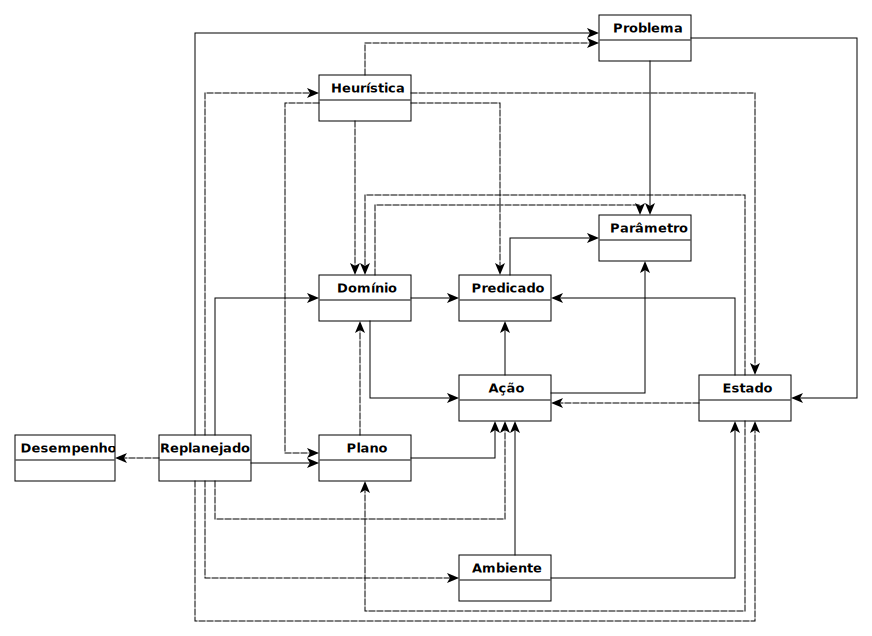
\includegraphics[angle=270,width=1.0\textwidth]{./img/diagrama_classe_sistema.ps}
    \caption[Diagrama de classe do sistema de reparo]{Diagrama de Classe\footnote{Este diagrama segue os conceitos apresentados por \cite{Martin2000}.} do sistema de reparo VHPOP-RE\index{VHPOP-RE}}
  \end{figure}
\end{center}


%%%%%%%%%%%%%%%%%%%%%%%%%%%%%%%%%%%%%%%%%%%%%%%%%%%%%%%%%%%%%%%%%%%%%%%%%

\onehalfspacing
\bibliographystyle{apalike}
\bibliography{diss-bib}

\printindex

\end{document}
